\documentclass[letterpaper, reqno,11pt]{article}
\usepackage[margin=1.0in]{geometry}
\usepackage{color,latexsym,amsmath,amssymb,graphicx,float,listings,tikz}
\usepackage{hyperref}

\hypersetup{
colorlinks=true,
linkcolor=magenta,
filecolor=magenta,
urlcolor=cyan,
}

\graphicspath{ {images/} }

\begin{titlepage}
\newgeometry{margin=3cm}
\centering

\vspace*{\stretch{2}}

\Large ELEC 302 Lab 3 Report

\vspace{\stretch{1}}

\normalsize Bipolar Junction Transistor and Amplifier

\vspace{\stretch{0.5}}

\begin{tabular}{ll}
Name & Xander Naumenko \\[2ex]
Student Number  & 38198354 \\[2ex]
Lab Group            & L2C \\[2ex]
Experiment Date            & 2023-03-18 \\[2ex]
Partner's Name &  Brian Sun
\end{tabular}

\vspace{\stretch{3}}


\vspace{\stretch{2}}
\end{titlepage}

{\medskip\noindent\bf Question 1.} From the prelab, we found that to achieve the target values, $R_c=200\Omega$ and $R_B=43k\Omega$. After putting these resistors in the circuit, the desired parameters were measured using the digital multimeter and can be seen in table \ref{tab:q1}. To get the currents, the voltages across $R_B$ and $R_C$ were measured then divided by their measured resistance values.

\begin{table}[htpb]
    \centering
    \caption{Measured values for Question 1.}
    \label{tab:q1}
    \begin{tabular}{|c|c|}
    \hline
    Parameter & Value \\
    $I_B$ & $99.3\mu $A \\
    $I_C$ & 16.5mA \\
    $V_{CE}$ & 1.75V \\
    \hline
    \end{tabular}
\end{table}

% $V_{R_B}=4.27V$, $V_{R_C}=3.29$, $V_{CE}=1.75$. $I_B=\frac{4.27}{43\cdot 10^{3}}=99.3\mu$A, $I_C=16.5$mA. $\beta=166.2$
From these values, we can get a value for $\beta$ by dividing the currents: $\beta = \frac{I_C}{I_B}=166.2$. See figure \ref{fig:q1} for the circuit diagram with the resistor parameters used.

\begin{figure}[htpb]
    \centering
    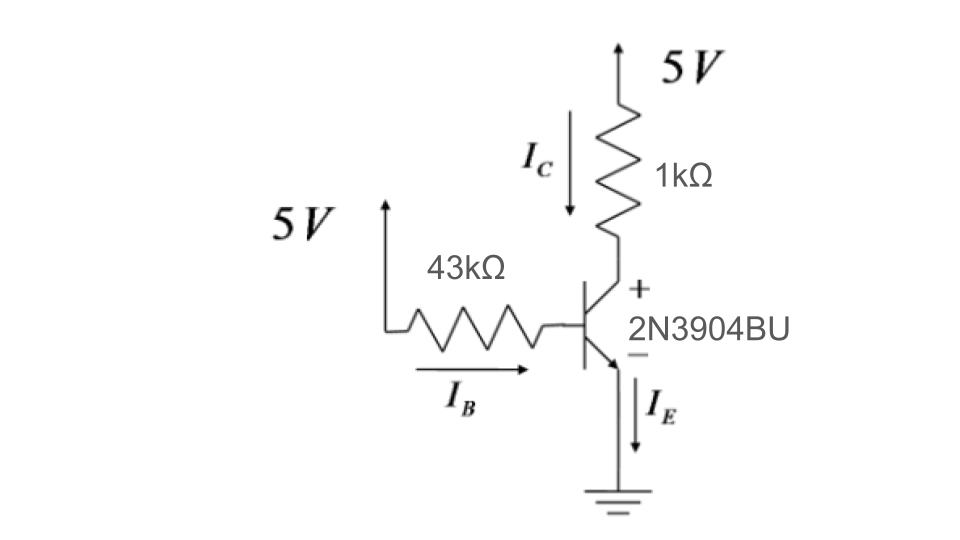
\includegraphics[width=0.8\textwidth]{q1}
    \caption{Circuit diagram for question 3. Mostly taken from the lab manual given it's the same circuit with the actual resistances used.}
    \label{fig:q1}
\end{figure}

{\medskip\noindent\bf Question 2.} Although the resistor values were previously calculated in the prelab, the value of $R$ must be changed given we now have a more accurate value for $\beta$ from part 1. Following the same approach as in the prelab:
\[
I_B=\frac{I_C}{\beta}=30.1\mu\text{A}
\]
\[
V_E=470\cdot \frac{\beta+1}{\beta} I_C=2.364\text{V}
\]
\[
10=2\cdot 2.364+R\cdot \frac{0.005}{166.2}\implies R=129k\Omega
.\]

Since we have to use resistor values we have, we used $R=130k\Omega$. $R_C$ is unaffected by $\beta$, so it is still $R_C=1k\Omega$. The circuit was assembled and the required values can be seen in table \ref{tab:q2}. As previously, the current values were determined by measuring the voltage across the resistors and dividing by the resistance.

\begin{table}[htpb]
    \centering
    \caption{Measured values for Question 2.}
    \label{tab:q2}
    \begin{tabular}{|c|c|}
    \hline
    Parameter & Value \\
    $I_C$ & 5.14mA \\
    $I_B$ & $29.2\mu $A \\
    $I_E$ & 5.19mA \\
    $V_{E}$ & 2.44V \\
    $V_{C}$ & 4.94V \\
    \hline
    \end{tabular}
\end{table}

See figure \ref{fig:q2} for the circuit diagram. The measured parameters weren't exactly what we were aiming for; $I_C$ was found to be 5.14mA instead of 5mA, and $V_C=4.94$V instead of 5V. These are both within 0.5\% of the desired values though, and a small variation is expected given we used a slightly different resistor value than we calculated due to availability.

% For the values: $V_{R_C}=5.14V\implies I_C=5.14$mA. $V_{R_E}=2.44\text{V}\implies I_E=5.19$mA. $V_{R_1}=6.93\text{V}, V_{R_2}=3.14\text{V}\implies I_B=29.15\mu$A, $V_C=4.94$

\begin{figure}[htpb]
    \centering
    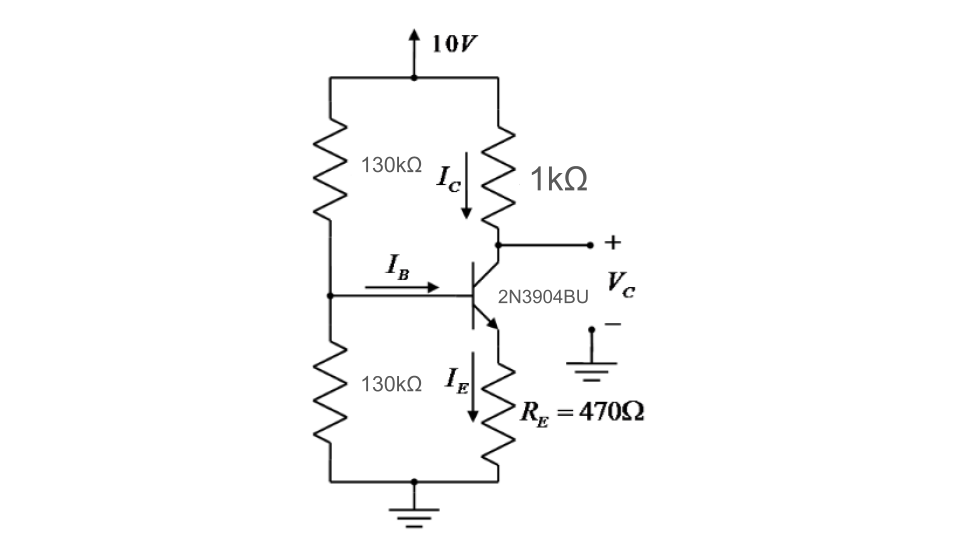
\includegraphics[width=0.8\textwidth]{q2}
    \caption{Circuit diagram for question 2. Again, the original circuit was taken from the prelab and changed to the specific values used.}
    \label{fig:q2}
\end{figure}

{\medskip\noindent\bf Question 3.} See figure \ref{fig:q3} for the input and output waveforms. From these graphs using the peak to peak voltages, we find that $A_v= \frac{v_0}{v_i}=-\frac{556}{40}=-13.9$ when the power supply is 10V, and $A_v=-\frac{496}{40}=-12.4$ for 4V supply. From the expressions derived in the prelab we wouldn't expect a change in gain for depending on the supply voltage, so this change is somewhat unexpected.

Likely the discrepancy comes from the small signal model and the assumptions invoked there. When deriving the gain originally we ignored the early effect, which does have power source dependence (since it involves adding $r_0=\frac{V_A}{I_C}$ to the hybrid $\pi$ model). We also assumed that the BJT is always in active mode, although this assumption seems true since we're operating well under the saturation range and we're not seeing any cutoff. Thus the early effect is the most likely culprit of this difference. %One key assumption in the small signal model is that the BJT is in active mode. To quickly check this assumption, assume that $V_{CE}=0.7$

\begin{figure}[htpb]
    \centering
    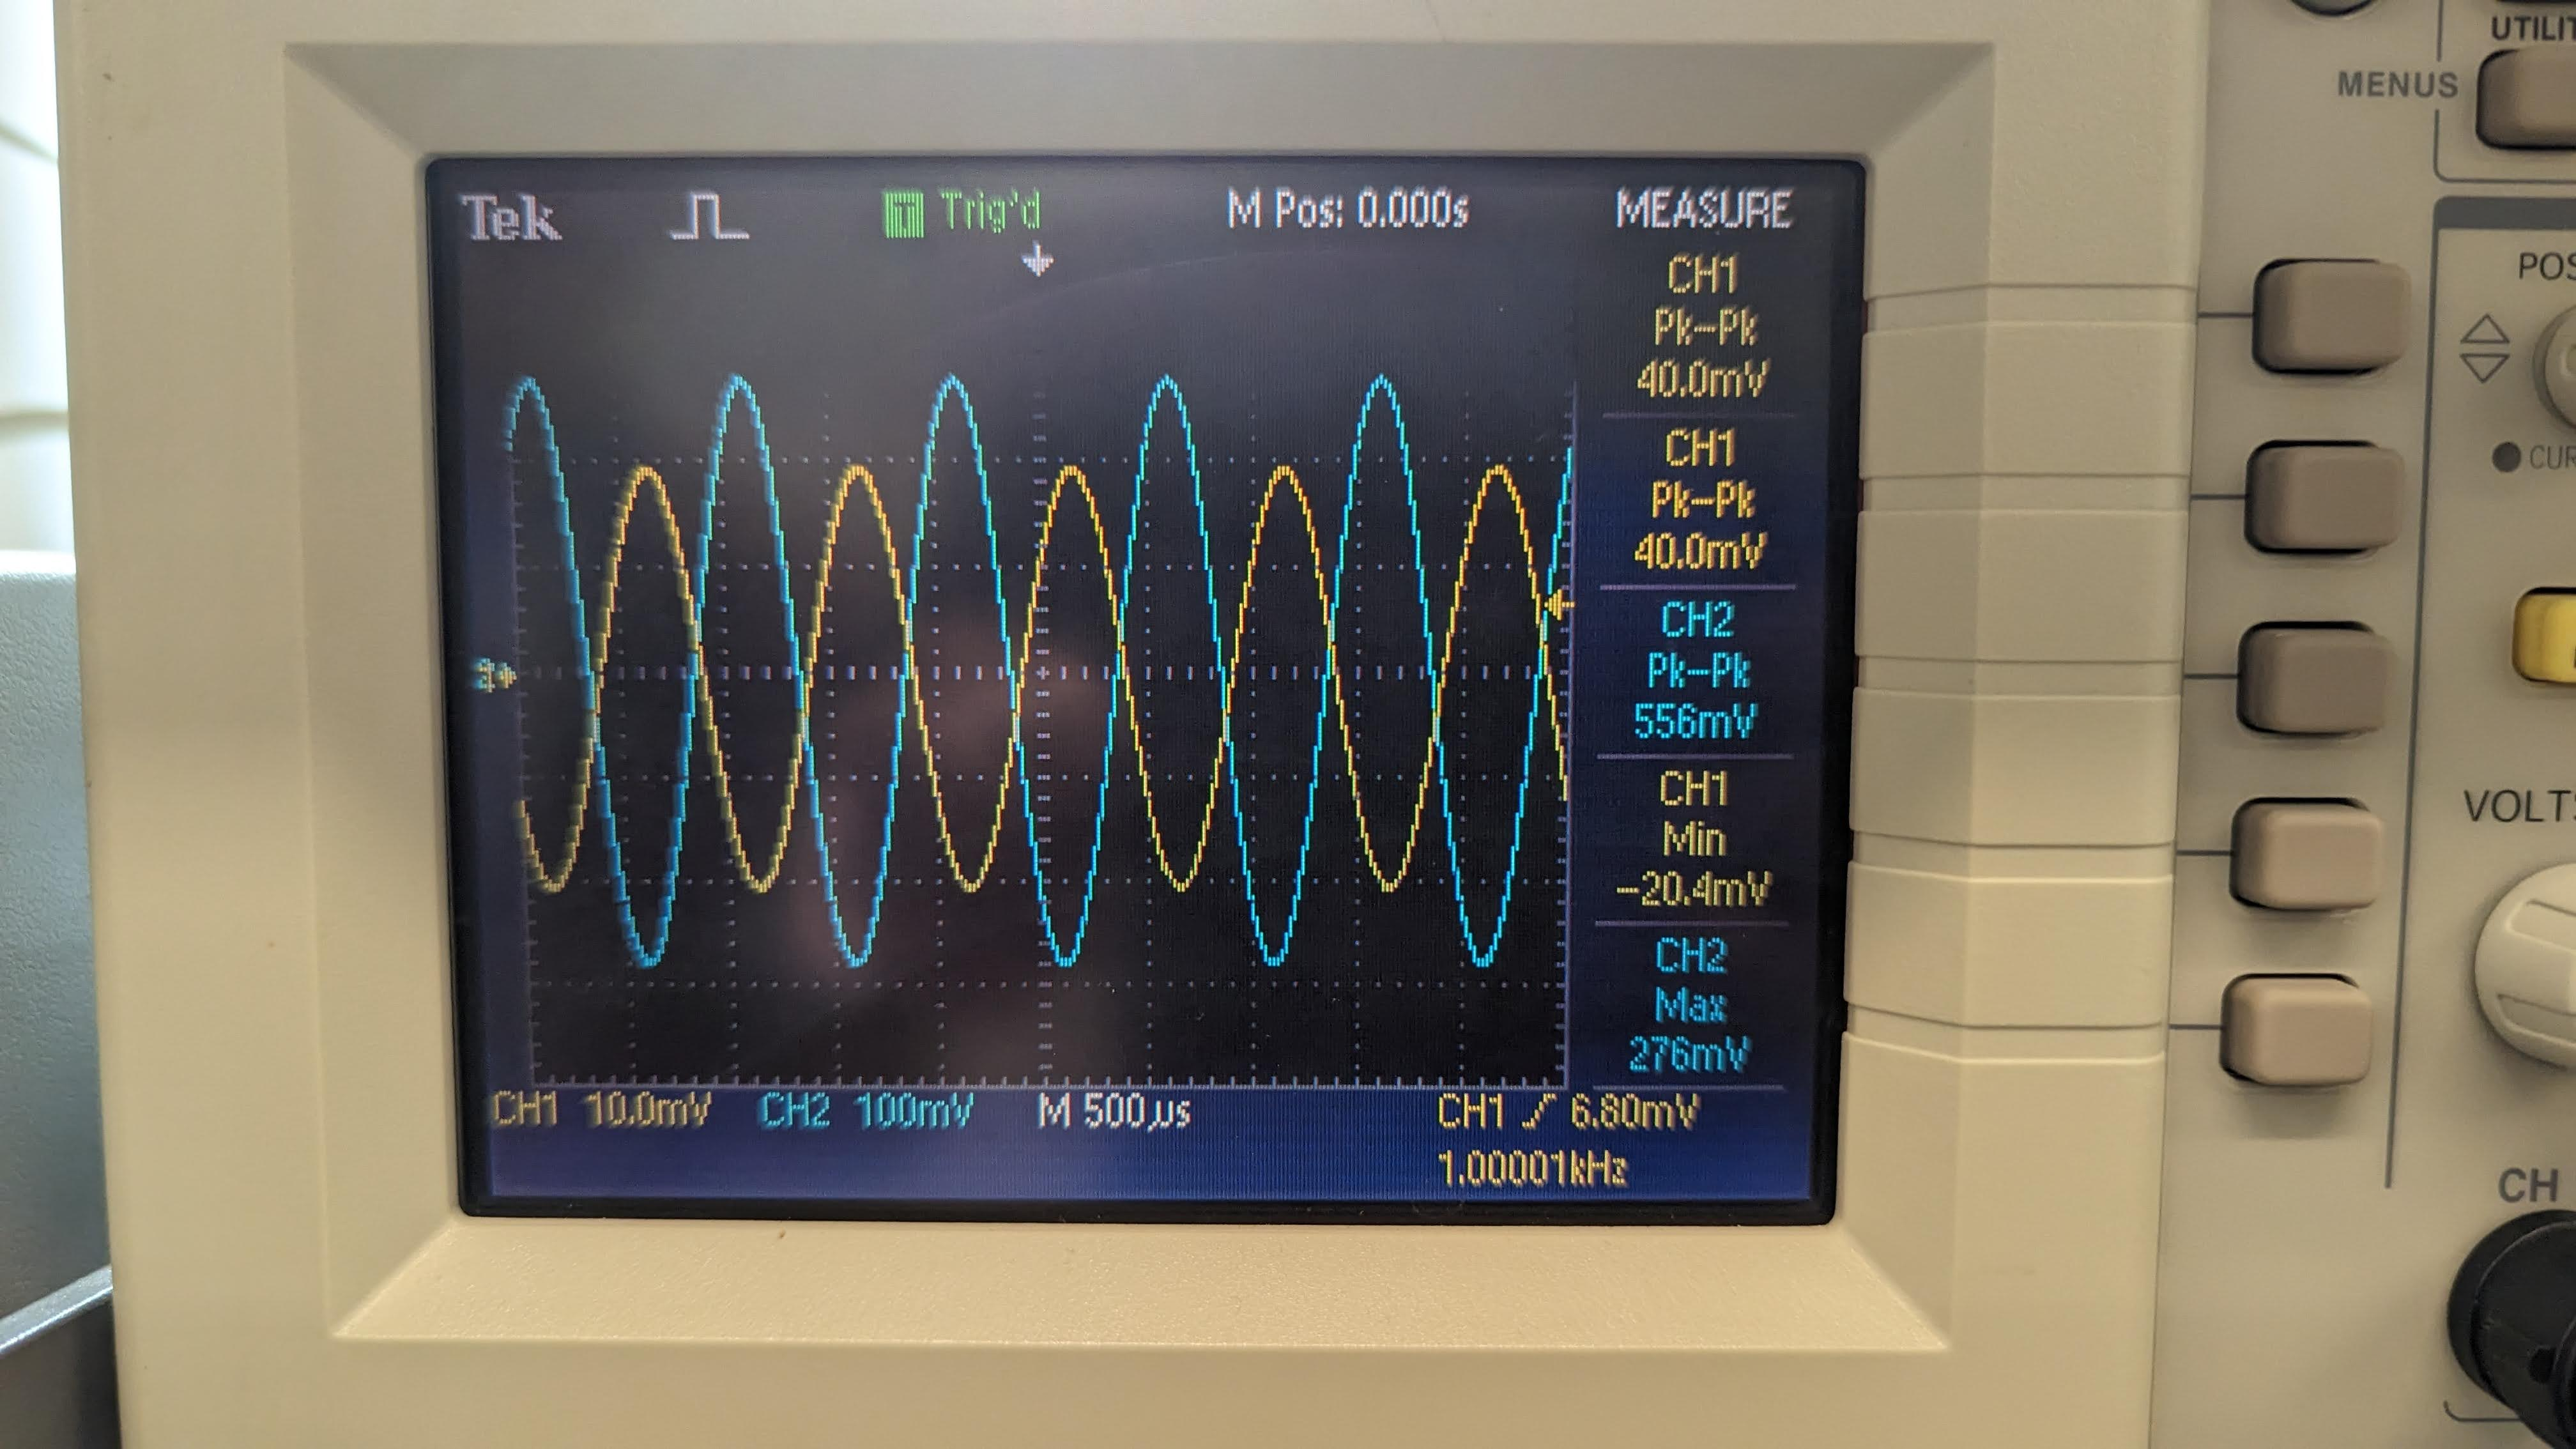
\includegraphics[width=0.49\textwidth]{q3-10}
    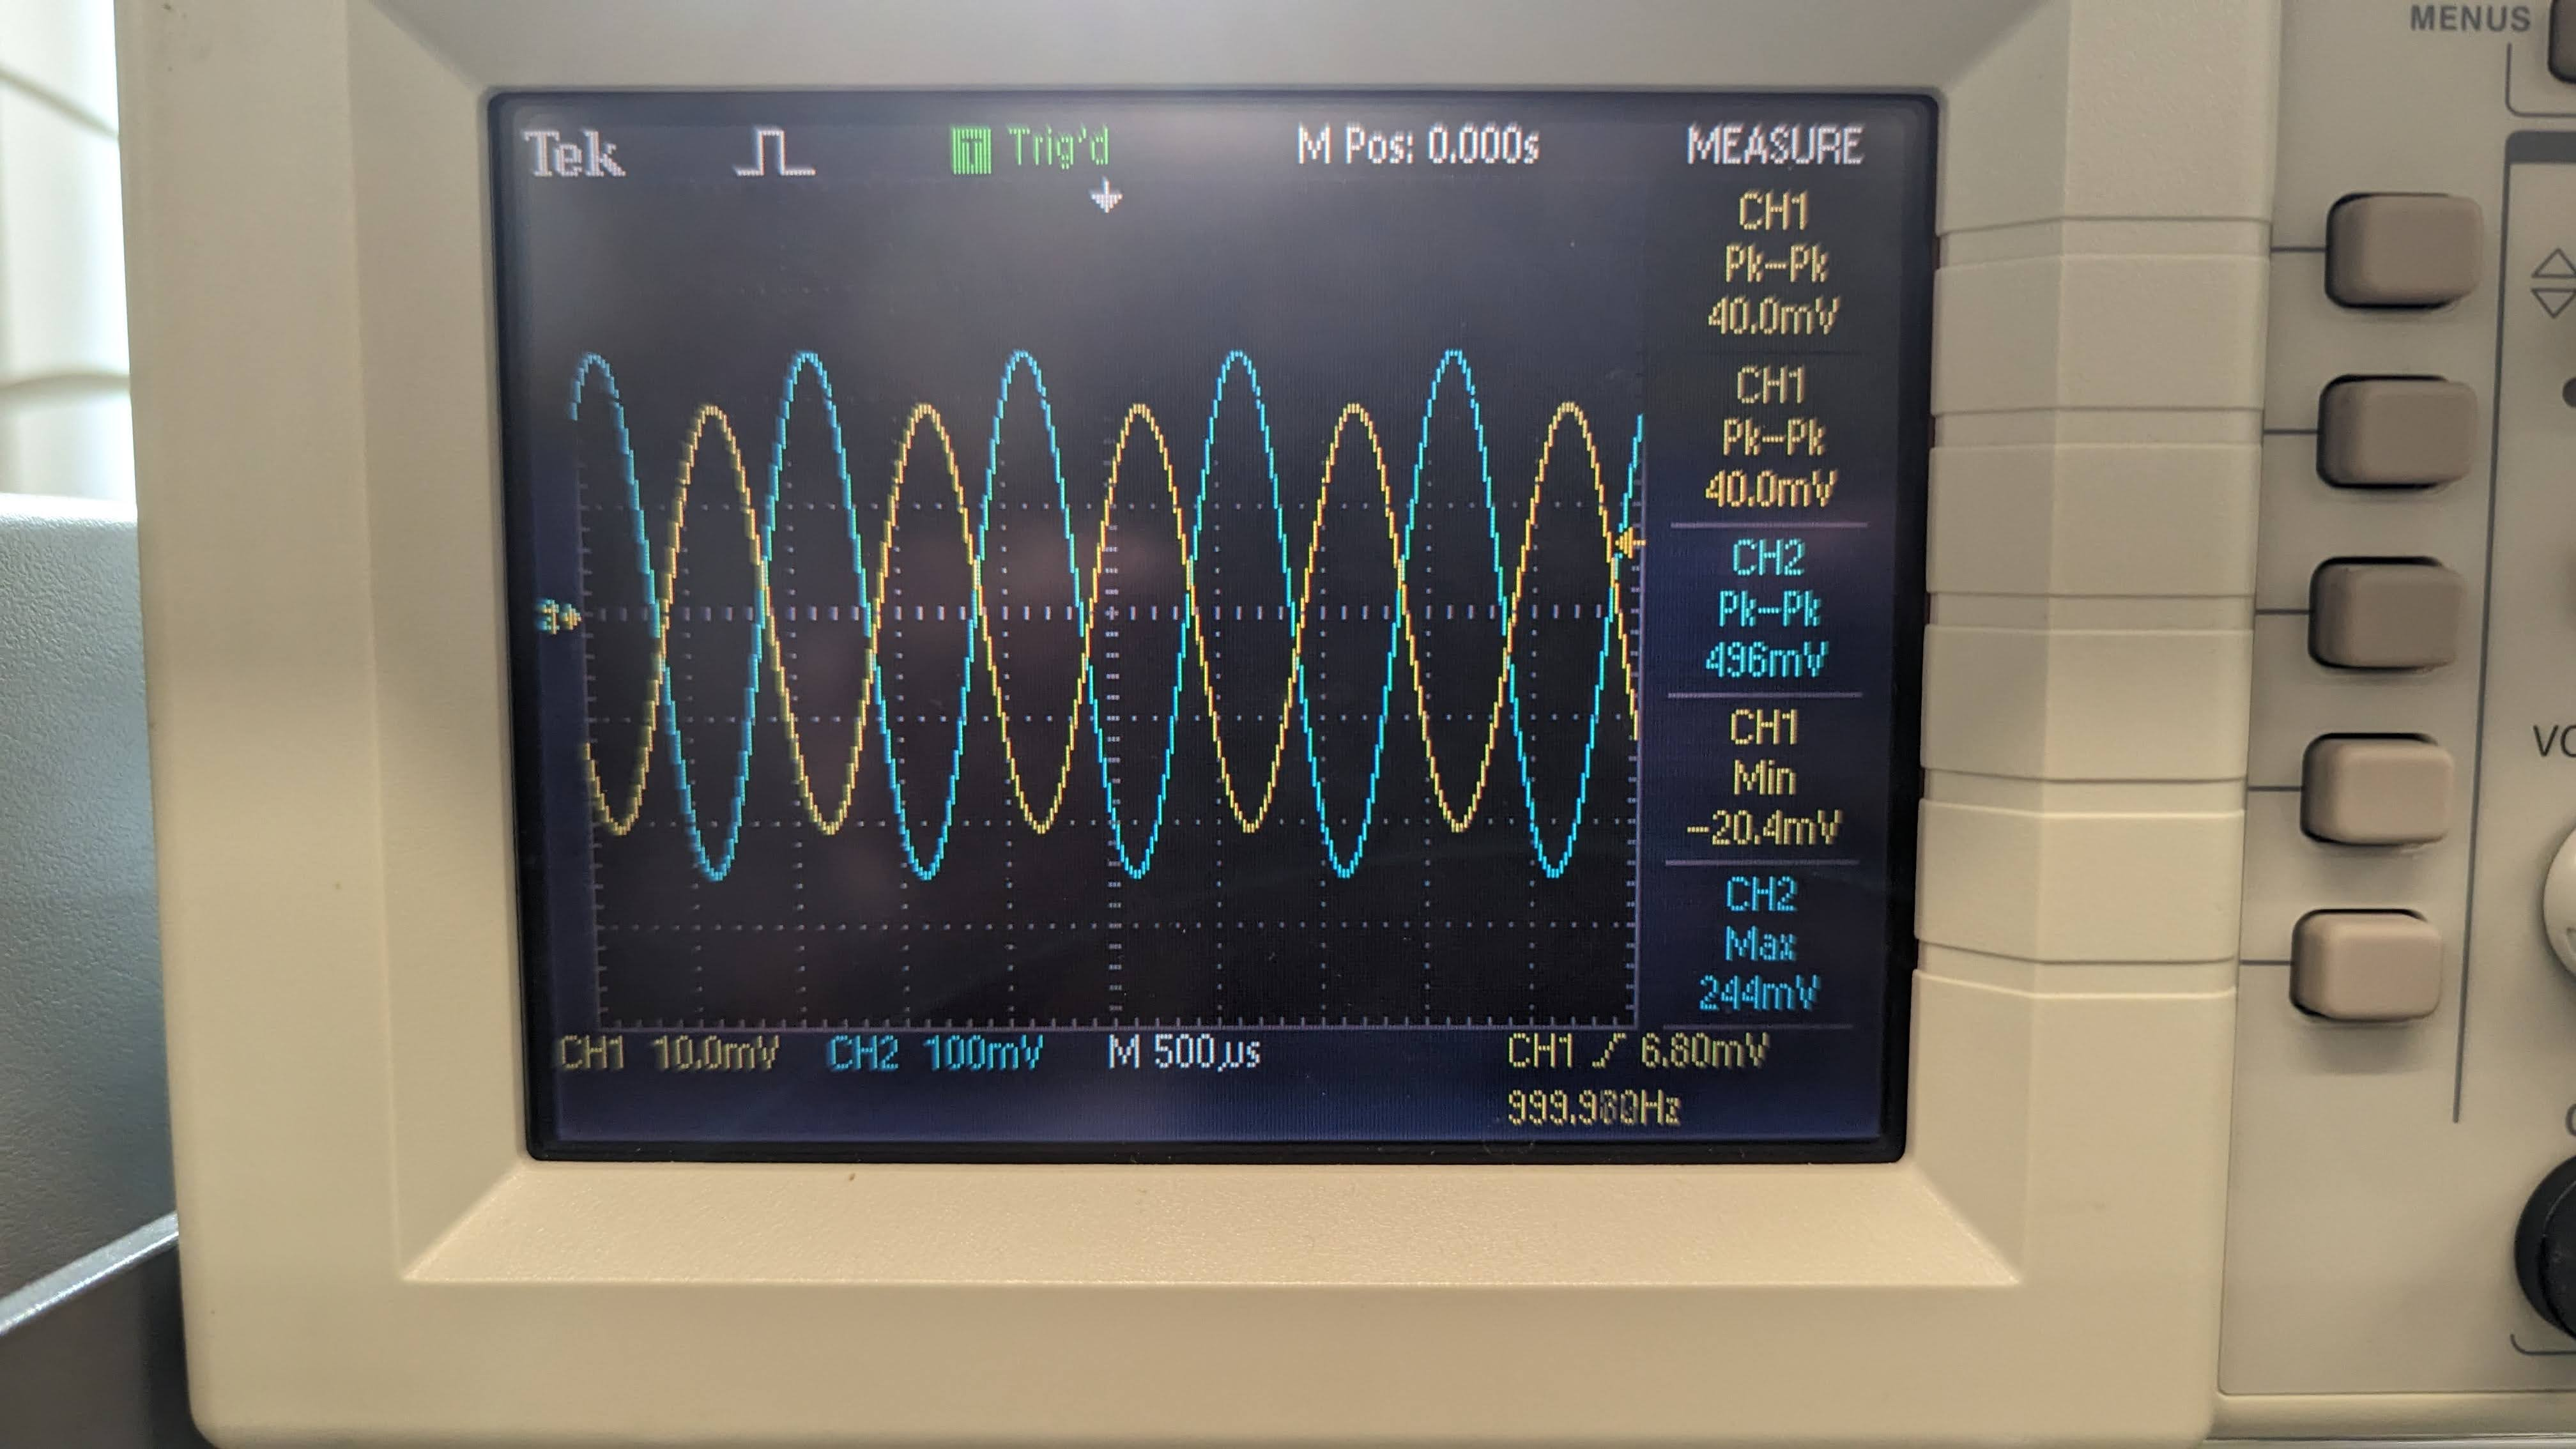
\includegraphics[width=0.49\textwidth]{q3-4}
    \caption{Input and output voltage waveforms for part 3. Left is 10V power supply, right is 4V. Yellow is the input waveform, and blue is the output waveform.}
    \label{fig:q3}
\end{figure}

For the theoretical value of $A_v$, we can use the same expression as the prelab:

\[
r_{\pi}= \frac{\beta}{g_m}=831\Omega\implies R_{in}= R_1 / / R_2 / / r_{\pi}=819.5\Omega
.\]
\[
v_o= -g_m v_{\pi} \left( R_C //R_L \right) = -g_m \left( v_i \frac{R_{in}}{R_S+R_{in}} \right) \left( R_C / / R_L \right)=-15v_i\implies A_v= \frac{v_o}{v_i}=-15
.\]
This is somewhat close to the $A_v=-13.9$ that we saw in the $10V$ supply case, although there's still around 1V of discrepancy. Originally we were having a lot of noise in the signal generator, but after switching signal generators most of the noise went away and we continued to see this value. As previously, it could be that the our neglecting of the early effect or other modeling choice changes the gain, as we saw that changing the power supply had an effect on this order of magnitude to the measured gain.



\end{document}
